\section{Norm und Spur}
Sei $L\mid K$ endliche Körpererweiterung und $\alpha \in L$.
\begin{remark}
	\proplbl{1_8_1}
	$L$ ist ein $K$-Vektorraum $\implies$ $\End_K (L)$ ist ein $K$-Vektorraum und ein (nicht kommutativer) Ring unter Komposition.
\end{remark}
\begin{definition}[Spur, Norm]
	\begin{enumerate}[label={(\alph*)}]
		\item 
		\bgroup
		\zeroAmsmathAlignVSpaces*[-0.5\baselineskip]
		\begin{flalign*}
		 \;\;&\mu_{\alpha}\colon \begin{cases}
		L & \to L\\
		x &\mapsto \alpha x
		\end{cases} \in \End_K (L) &
		\end{flalign*}
		\egroup
		\item \begin{enumerate}[label=,left=0pt]
			\item $N_{L \mid K}(\alpha) := \det(\mu_{\alpha}$, die $(L \mid K)$- Norm von $\alpha$
			\item $\Tr_{L \mid K}(\alpha) := \Tr(\mu_{\alpha})$, die $(L\mid K)$-Spur von $\alpha$
		\end{enumerate}
		\item \begin{enumerate}[label=,left=0pt]
			\item $\chi_{\alpha} :=$ charakteristisches Polynom von $\mu_{\alpha}$
			\item $f_{\alpha} :=$ Minimalpolynom von $\mu_{\alpha}$
		\end{enumerate}
	\end{enumerate}
\end{definition}
\begin{lemma}
	\proplbl{1_8_3}
	\begin{enumerate}[label={(\alph*)}]
		\item $f_{\alpha} = \MinPol(\alpha \mid K)$
		\item $\chi_{\alpha} = f_{\alpha}^m$ für $m = [L:K(\alpha)]$
	\end{enumerate}
\end{lemma}
\begin{proof}\leavevmode
	\begin{enumerate}[topsep=-6pt,left=0pt,label={(\alph*)}]
		\item Die Abbildung
		\begin{flalign*}
			\quad&\mu\colon \left\lbrace\begin{array}{@{}l@{\;}c@{\;}l}
			L & \to &\End_K(L)\\
			\beta & \mapsto& \mu_{\beta} 
			\end{array}\right. & \tag{$\star$} \proplbl{bew:1_8_3}
		\end{flalign*}
		ist $K$-linearer Ringhomomorphismus: \checkmark\\
		Sei $g:= \MinPol(\alpha \mid K)$. Dann
		\begin{flalign*}
			\quad &\left.\begin{array}{@{}l@{\,}c@{\,}l@{\;}l@{\;}l@{\;\;}c@{\;\;}l@{\;}l}
			g(\mu_{\alpha}) & \overset{\eqref{bew:1_8_3}}{=} & \mu_{g(\alpha)} & = & 0 \in \End_K(L) &&& \implies  f_{\alpha}\mid g\\
			\mu_{f_{\alpha}(\alpha)} & \overset{\eqref{bew:1_8_3}}{=} & f_{\alpha}(\mu_{\alpha}) & = & 0 \in \End_K(L) & \xRightarrow{\mu \text{ inj.}} & f_{\alpha}(\alpha) = 0 & \implies g \mid f_{\alpha}
			\end{array}\right\rbrace \implies f_{\alpha} = g &
		\end{flalign*}
		\item Charakteristisches Polynom und Minimalpolynom haben die gleichen irreduziblen Faktoren: $\nearrow$ LAAG VIII.7.6 oder direkt:
		\vspace*{\dimexpr-\baselineskip-2\lineskip}
		\begin{adjustwidth}{1.5em}{0pt}
			\item $V$ $n$-dimensionaler $K$-VR, $\varphi \in \End_K(V)$, $\mathscr{B}$ Basis von $V$ $\rightsquigarrow$ $A = M_{\mathscr{B}}(f)$. $\chi_{\varphi} = \chi_A \in K[X]$ zerfällt in Linearfaktoren in $\bar{K}[X]$\\
			$\implies$ lese $\chi_{\varphi} = \chi_A \und P_{\varphi} = P_A$ aus der Jordan-Normalform von $A$ ab.
		\end{adjustwidth}
		$f_{\alpha} = \MinPol(\alpha\mid K)$ irreduzibel $\implies \chi_{\alpha} = f_{\alpha}^m$ für ein $m$ und
		\begin{flalign*}
			\quad&\left .\begin{array}{@{}l@{\,}c@{\,}l@{\,}c@{\,}l}
			\deg(f_{\alpha}) &=& \deg(\alpha \mid K) &=& [K(\alpha) : K]\\
			\deg(\chi_{\alpha}) &=& \mathrm{dim}_{\mathrm K}\, L &=& [L:K]	
			\end{array}\right\rbrace \implies m = \frac{\deg(\chi_{\alpha})}{\deg(f_{\alpha})} = \frac{[L:K]}{[K(\alpha):K]} = [L:K(\alpha)] &
		\end{flalign*}
	\end{enumerate}
\end{proof}
\begin{example}
	\proplbl{1_8_4}
	Sei $\C = \R + \R\ii$, $\alpha = x+y\ii \in \C$.
	\begin{itemize}[topsep=-6pt]
		\item[$\Rightarrow$] $\mu_\alpha$ bezüglich Basis $(1,i) = \mathcal B$ ist \begin{flalign*}
			\quad & M_{\mathcal B}(\mu_\alpha) = \begin{pmatrix}
				x & -y \\ y & x
			\end{pmatrix} &
		\end{flalign*}
		\item[$\Rightarrow$] $\begin{aligned}[t]N_{\mathbb C\mid\mathbb R} (\alpha)\; &= \det\big(M_{\mathcal B}(\mu_\alpha)\big) = x^2 + y^2 = \vert \alpha\vert^2 = \alpha\bar\alpha,\\
		\mathrm{Sp}_{\mathbb C\mid\mathbb R}(\alpha) &= \mathrm{Sp}\big( M_{\mathcal B}(\mu_\alpha)\big) = 2\alpha = \alpha + \bar\alpha\end{aligned}$\\[4\lineskip]
		$\begin{aligned}[t]\chi_\alpha(t) &= \det(\mathbbm 1 - A) = (t - x)^2 + y^2 = t^2- 2xt + x^2 + y^2 = t^2 - 2 \mathrm{Sp}_{\mathbb C\mid\mathbb R}(\alpha)t + N_{\mathbb C\mid\mathbb R}(\alpha)\\
		& = (t - \alpha)(x - \bar\alpha),\\
		\displaystyle f_\alpha(t) &= \begin{cases}
			t - \alpha, & \alpha\in\mathbb R,\\ (t-\alpha)(t-\bar\alpha), & \alpha\notin\mathbb R
		\end{cases}\end{aligned}$
	\end{itemize}
\end{example}

\begin{lemma}
	\proplbl{1_8_5}
	Seien $n = [L:K]$ und $\alpha$,$\beta\in L$, $\lambda\in K$.
	\begin{enumerate}[label={(\alph*)}]
		\item $N_{L\mid K}(\alpha\beta) = N_{L\mid K}(\alpha)\cdot N_{L\mid K}(\beta)$,
		\item $\mathrm{Sp}_{L\mid K}(\lambda\alpha + \beta) = \lambda\,\mathrm{Sp}_{L\mid K}(\alpha) + \mathrm{Sp}_{L\mid K}(\beta)$,
		\item $N_{L\mid K}(\lambda) = \lambda^n$, $\mathrm{Sp}_{L\mid K}(\lambda) = n\cdot\lambda$,
		\item Ist $f_\alpha = X^r + a_{r-1} X^{r-1} + \dots + a_0$ und $m = [L:K(\alpha)] = n\mskip-1mu\big\slash \mskip-1mu r$, so ist \begin{flalign*}
			\quad & N_{L\mid K}(\alpha) = (-1)^n a_0^m,\quad\mathrm{Sp}_{L\mid K}(\alpha) = -m a_{r-1} &
		\end{flalign*}
	\end{enumerate}
\end{lemma}
\begin{proof}\leavevmode
	\begin{itemize}[topsep=-6pt,widest={(a), (b)},leftmargin=*]
		\item[(a), (b)] klar: Multiplikativität der Determinante und Linearität der Spur
		\item[(c)] $M_{\mathcal B}(\mu_\lambda) = \lambda\mathbbm 1$ für alle Basen $\mathcal B$ von $L$.
		\item[(d)] $\chi_\alpha = X^n + b_{n-1} X^{n-1} + \dots + b_0$ \begin{itemize}[topsep=-6pt]
			\item[$\Rightarrow$] $\det\mu_\alpha = (-1)^n \chi_\alpha(0) = (-1)^n b_0$, $\mathrm{Sp}_{\mu_\alpha} = - b_{n-1}$
		\end{itemize}
		\vspace*{4\lineskip}
		$\chi_\alpha = \big(f_{\alpha}\big)^m$
		\begin{itemize}[topsep=-6pt]
			\item[$\Rightarrow$] $N_{L\mid K}(\alpha) = \det(\mu_\alpha) = (-1)^n a_0^m$, $\mathrm{Sp}_{L\mid K}(\alpha) = \mathrm{Sp}\,\mu_\alpha = -b_{n-1} = -m \cdot a_{n-1}$
		\end{itemize}
	\end{itemize}
\end{proof}

\begin{remark}
	\proplbl{1_8_6}
	\begin{enumerate}[left=0pt,label={(\alph*)}]
		\item Ist $\alpha$ inseparabel über $K$, so ist $f_\alpha(X) = g(X^r)$ für ein $g\in K[X]$, und somit ist \begin{flalign*}
			\quad & \mathrm{Sp}_{L\mid K}(\alpha) = -m\cdot \underbrace{a_{r-1}}_{=0} = 0 &
		\end{flalign*}
		\item Ist $L\mid K(\alpha)$ inseparabel, so ist $m = p^d\cdot [L:K(\alpha)]_{\mathrm S}$, somit ist ist \begin{flalign*}
			\quad & \mathrm{Sp}_{L\mid K}(\alpha) = \underbrace{m}_{\mathclap{=0}}\cdot\, a_{r-1} = 0 &
		\end{flalign*}
		\item Aus $(a)$ und $(b)$ folgt: \begin{adjustwidth}{2em}{0pt}
			$L\mid K$ inseparabel \hspace*{1em} $\Leftrightarrow$ \hspace*{1em} $\mathrm{Sp}_{L\mid K} = 0$
		\end{adjustwidth}
	\end{enumerate}
\end{remark}

\begin{proposition}
	\proplbl{1_8_7}
	Ist $\alpha\in L$, $n=[L:K] = q\cdot r$ und $r=[L:K]_{\mathrm S}$ sowie $\hom_K(L,\bar K) = \{ \sigma_1,\dots,\sigma_r \}$, so gilt \begin{flalign*}
		\quad & N_{L\mid K}(\alpha) = \Bigg( \prod_{r=1}^n \sigma_j(\alpha)\Bigg)^q,\qquad \mathrm{Sp}\,(\alpha) = q\sum_{i=1}^{r} \sigma_i(\alpha) &
	\end{flalign*}
\end{proposition}
\begin{proof}\leavevmode\\[2pt]
	\begin{minipage}{0.5\linewidth}
	Sei $n_1 = [K(\alpha): K] = r_1 q_1$ und $n_2 = [L:K(\alpha)] = r_2 q_2$. Schreibe \begin{flalign*}
		\quad & f_\alpha = X^{r_1} + a_{n_1 - 1} X^{n_1 - 1} + \dots + a_0 = \prod_{i=1}^{r_1} \big( X - \tau_i(\alpha)\big)^{q_1} = g\big( X^{q_1}\big),&\\
		&g(X) = \prod_{i=1}^{r_1} \big( X - \tau_i^{q_1}(\alpha)\big) &
	\end{flalign*}
	\smallskip
	\end{minipage}%
	\hfill%
	\begin{minipage}{0.49\linewidth}
	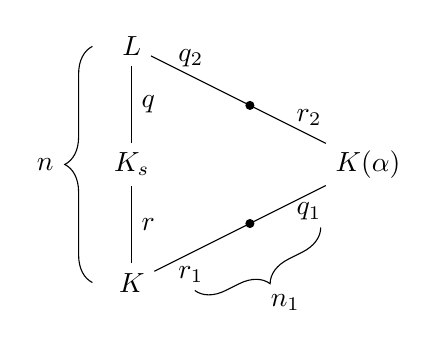
\begin{tikzpicture}
	\node at (0,0) (L) {$L$};
	\node at (0,-1.5) (KS) {$K_s$};
	\node at (0,-3) (K) {$K$};
	\node at (3,-1.5) (Kalpha) {$K(\alpha)$};
	
	\draw (L) to node [right] {$q$} (KS);
	\draw (KS) to node [right] {$r$} (K);
	\draw (L) -- (Kalpha);
	\draw (K) -- (Kalpha);
	\draw[fill=black] (1.5,-0.75) circle (0.05);
	\draw[fill=black] (1.5,-2.25) circle (0.05);
	
	\draw [decorate,decoration={brace,amplitude=10pt,mirror},xshift=-0.5cm,yshift=0pt]
	(0,0) -- (0,-3) node [black,midway, xshift=-0.6cm]{$n$};
	
	\node at (0.75,-0.15) (q2) {$q_2$};
	\node at (0.75,-2.9) (r1) {$r_1$};
	\node at (2.25,-0.9) (r2) {$r_2$};
	\node at (2.25,-2.1) (q1) {$q_1$};
	
	\draw [decorate,decoration={brace,amplitude=10pt,mirror}]
	(0.8,-3.1) -- (2.4,-2.3);
	\node at (1.95,-3.25) (n1) {$n_1$};
	\end{tikzpicture}
	\end{minipage}
	Jedes $\tau_i$ hat genau $r_2$ viele Fortsetzungen zu einem $\sigma_j \in \hom_K(L\mid \bar K)$ (\propref{1_7_3}), sodass \begin{flalign*}
	\quad & \Bigg(\prod_{j=1}^r \sigma_j(\alpha)\Bigg)^q = \Bigg( \prod_{i=1}^{r_1} \tau_i(\alpha)^{r_2}\Bigg)^q = \big( (-1)^{r_1} a_0\big)^{r_2 q_2} = (-1)^n a_0^{r_2} \overset{\propref{1_8_5}}{=} N_{L\mid K}(\alpha), \\
	& q\sum_{i=1}^r \sigma_j(\alpha) = q r_2 \sum_{i=1}^{r_1} \tau_j(\alpha) = - q_2 r_1 a_{n_1 - 1} = \mathrm{Sp}_{L\mid K}(\alpha) &
	\end{flalign*}
\end{proof}

%to add 16 May 2019 %TODO
\begin{lemma}
	\proplbl{1_8_8}
	Seien $K \subseteq L \subseteq M$ Körper mit $M\mid K$ endlich und sei $\alpha\in M$. Dann ist
	\begin{itemize}
		\item $N_{M \mid K}(\alpha) = N_{L\mid K}\big(N_{M\mid L}(\alpha)\big)$
		\item $\Tr_{M \mid K}(\alpha) = \Tr_{L \mid K}\big(\Tr_{M \mid L}(\alpha)\big)$
	\end{itemize}
\end{lemma}
\begin{proof}
	Sei $[L:K] = q_1 \cdot r_1$, $[M:L] = q_2 \cdot r_2$; $\Hom(M, \bar{L}) = \set{\sigma_1, \dots, \sigma_{r_2}}$. Fixiere die Einbettung $L \subseteq \bar{K}$ und setze $\tau_i$ fort zu $\tilde{\tau}_i \in \Aut(\bar{K}\mid K)$( \propref{1_4_11}) %TODO
	Dann ist
	\begin{flalign*}
		\quad & \Hom_K(M, \bar{K}) = \big\lbrace \tilde{\tau}_i \circ \sigma_j\;\big|\; i =1, \dots, r_1,\; j = 1, \dots, r_2\big\rbrace, &
	\end{flalign*}
	denn $\# \Hom(M, \bar{K}) = [M: K]_{\mathrm S} = r_1 \cdot r_2$ und
	\begin{flalign*} %TODO check for { } misssing
		\quad & \begin{aligned}[t]
			& \tilde \tau_i\circ \sigma_j = \tilde \tau_{i'}\circ\sigma_{j'} \\
			\Rightarrow \;& \sigma_j = \big( \tilde \tau_i^{-1}\circ \tilde\tau_{i'}\big)\circ \sigma_{j'} \\
			\Rightarrow\; & \tilde \tau_i^{-1} \circ \left. \tilde \tau_i \right| _{L} = \id_L \\
			\Rightarrow\; & \tau_i = \tau_{k'} \quad \Rightarrow i=i' \quad \Rightarrow \sigma_j = \sigma_{j'} \quad\Rightarrow j = j' \\
			\Rightarrow\; & N_{L\mid K}\big( N_{M\mid L}(\alpha)\big) \overset{\propref{1_8_7}}{=} N_{L\mid K}\Bigg( \prod_{j=1}^{r_2} \sigma_i(\alpha) \Bigg)^{q_2} \overset{\propref{1_8_7}}{=} \prod_{i=1}^{r_1} \tilde \tau_i \Bigg( \prod_{j=1}^{r_2} \sigma_j(\alpha)\Bigg)^{q_1 q_2} = \Bigg( \prod_{i,j} \big(\tilde \tau_i \circ\sigma_j\big)(\alpha)\Bigg)^{q_1 q_2} \overset{\propref{1_8_7}}{=} N_{M\mid K}(\alpha)
		\end{aligned} &
	\end{flalign*}
	Analog für die Spur.
\end{proof}
\begin{theorem}[Unabhängigkeit der Charaktere, \person{Artin}]
	\proplbl{1_8_9}
	Sei $G$ eine Gruppe. Sind $\chi_1, \dots, \chi_n \in \Hom(G, K^{\times})$ paarweise verschieden, so sind sie linear unabhängig im $K$-Vektorraum $\Abb(G,K)$.
\end{theorem}
\begin{proof} %TODO reformat!
	Seien $\chi_1, \dots, \chi_n$ linear abhängig, oE $n \ge 2$ minimal, d.h.
	\begin{flalign*}
		\quad & \sum_{i=1}^n a_i \chi_i = 0 \quad\text{mit}\; a_1, \dots, a_n \in K^{\times}. &
	\end{flalign*}
	Sind $\chi_1 \neq \chi_n$ $\implies$ $\exists g \in G$ mit $\chi_1(g) \neq \chi_n(g)$. Ist die Summe $\sum a_i \chi_i = 0$, so  folgt, dass $\forall h \in G$ ist $\sum_{i=1}^n a_i \chi_i (h) = 0$ und
	\begin{flalign*}
		\quad & \begin{aligned}[t]
		\implies & \forall h\in G\colon\;\left\lbrace\begin{array}{@{}l@{\,}c@{\,}l}
			\sum_{i=1}^n a_i \cdot \underbrace{\chi_i (hg)}_{\chi_i(h)\cdot \chi_i(g)} &=& 0\\
			\sum_{i=1}^n a_i \cdot \chi_i(h)\cdot \chi_i(g) &=& 0
		\end{array}\right.\\
		\implies & 0 = \sum_{i=1}^n a_i \cdot \chi_i(h)\big(\chi_i(g) - \chi_n(g)\big) = \sum_{i=1}^{n-1} a_i \big(\chi_i(g) - \chi_n(g)\big)\cdot \chi_i(h)\\
		\implies & \sum_{i=1}^{n-1} a_i \cdot \big(\chi_i(g) - \chi_n(g)\big)\cdot \chi_i = 0
	\end{aligned} &
	\end{flalign*}
	$
	a_n (\chi_1(g) - \chi_n(g)) \neq 0$, was ist ein Widerspruch zur Minimalität von $n$.
\end{proof}
\begin{conclusion}
	\proplbl{1_8_10}
	Genau dann ist $\Tr_{L \mid K} \neq 0$, wenn $L \mid K$ separabel.
\end{conclusion}
\begin{proof}\leavevmode
	\begin{itemize}[topsep=-6pt]
		\item[($\Rightarrow$)] \propref{1_8_6}
		\item[($\Leftarrow$)] Sei $\Hom_K(L, \bar{K}) = \set{\sigma_1, \dots, \sigma_n}$. $\left.\sigma_i\right|_{L^{\times}} \in \Hom_K(L^{\times}, K^{\times})$\\
		$\xRightarrow{\propref{1_8_7}}$ $\sigma_1,\dots, \sigma_n$ sind $\bar{K}$-linear unabhängig. Insbesondere ist $\Tr_{L \mid K} = \sum_{i=1}^n \sigma_i \neq 0$.
	\end{itemize}
\end{proof}